\documentclass{beamer}
\usepackage[T1]{fontenc}
\usepackage[brazilian]{babel}
\usepackage{csquotes}
\usepackage[backend=biber,style=abnt,accite,extradate]{biblatex}
\addbibresource{referencias.bib}
\defbibenvironment{bibliography}{\list{}{\setlength{\leftmargin}{\bibhang}\setlength{\itemindent}{-\leftmargin}\setlength{\itemsep}{0.5em}\setlength{\parsep}{0pt}\setlength{\topsep}{0pt}}}{\endlist}{\item}
\renewcommand*{\bibfont}{\tiny}
\setbeamertemplate{bibliography item}{}
\setbeamertemplate{frametitle continuation}[from second]
\usepackage{fvextra}
\usepackage{tcolorbox}
\newtcolorbox{nixbox}[1]{colback=black!4,colframe=black!35,boxrule=0.4pt,arc=1pt,coltitle=white,colbacktitle=black!55,fonttitle=\ttfamily\scriptsize,title=#1,left=13pt,right=1pt,top=2pt,bottom=2pt,boxsep=1pt}

\makeatletter
\def\PY@reset{\let\PY@it=\relax \let\PY@bf=\relax%
    \let\PY@ul=\relax \let\PY@tc=\relax%
    \let\PY@bc=\relax \let\PY@ff=\relax}
\def\PY@tok#1{\csname PY@tok@#1\endcsname}
\def\PY@toks#1+{\ifx\relax#1\empty\else%
    \PY@tok{#1}\expandafter\PY@toks\fi}
\def\PY@do#1{\PY@bc{\PY@tc{\PY@ul{%
    \PY@it{\PY@bf{\PY@ff{#1}}}}}}}
\def\PY#1#2{\PY@reset\PY@toks#1+\relax+\PY@do{#2}}

\@namedef{PY@tok@w}{\def\PY@tc##1{\textcolor[rgb]{0.73,0.73,0.73}{##1}}}
\@namedef{PY@tok@c}{\let\PY@it=\textit\def\PY@tc##1{\textcolor[rgb]{0.24,0.48,0.48}{##1}}}
\@namedef{PY@tok@cp}{\def\PY@tc##1{\textcolor[rgb]{0.61,0.40,0.00}{##1}}}
\@namedef{PY@tok@k}{\let\PY@bf=\textbf\def\PY@tc##1{\textcolor[rgb]{0.00,0.50,0.00}{##1}}}
\@namedef{PY@tok@kp}{\def\PY@tc##1{\textcolor[rgb]{0.00,0.50,0.00}{##1}}}
\@namedef{PY@tok@kt}{\def\PY@tc##1{\textcolor[rgb]{0.69,0.00,0.25}{##1}}}
\@namedef{PY@tok@o}{\def\PY@tc##1{\textcolor[rgb]{0.40,0.40,0.40}{##1}}}
\@namedef{PY@tok@ow}{\let\PY@bf=\textbf\def\PY@tc##1{\textcolor[rgb]{0.67,0.13,1.00}{##1}}}
\@namedef{PY@tok@nb}{\def\PY@tc##1{\textcolor[rgb]{0.00,0.50,0.00}{##1}}}
\@namedef{PY@tok@nf}{\def\PY@tc##1{\textcolor[rgb]{0.00,0.00,1.00}{##1}}}
\@namedef{PY@tok@nc}{\let\PY@bf=\textbf\def\PY@tc##1{\textcolor[rgb]{0.00,0.00,1.00}{##1}}}
\@namedef{PY@tok@nn}{\let\PY@bf=\textbf\def\PY@tc##1{\textcolor[rgb]{0.00,0.00,1.00}{##1}}}
\@namedef{PY@tok@ne}{\let\PY@bf=\textbf\def\PY@tc##1{\textcolor[rgb]{0.80,0.25,0.22}{##1}}}
\@namedef{PY@tok@nv}{\def\PY@tc##1{\textcolor[rgb]{0.10,0.09,0.49}{##1}}}
\@namedef{PY@tok@no}{\def\PY@tc##1{\textcolor[rgb]{0.53,0.00,0.00}{##1}}}
\@namedef{PY@tok@nl}{\def\PY@tc##1{\textcolor[rgb]{0.46,0.46,0.00}{##1}}}
\@namedef{PY@tok@ni}{\let\PY@bf=\textbf\def\PY@tc##1{\textcolor[rgb]{0.44,0.44,0.44}{##1}}}
\@namedef{PY@tok@na}{\def\PY@tc##1{\textcolor[rgb]{0.41,0.47,0.13}{##1}}}
\@namedef{PY@tok@nt}{\let\PY@bf=\textbf\def\PY@tc##1{\textcolor[rgb]{0.00,0.50,0.00}{##1}}}
\@namedef{PY@tok@nd}{\def\PY@tc##1{\textcolor[rgb]{0.67,0.13,1.00}{##1}}}
\@namedef{PY@tok@s}{\def\PY@tc##1{\textcolor[rgb]{0.73,0.13,0.13}{##1}}}
\@namedef{PY@tok@sd}{\let\PY@it=\textit\def\PY@tc##1{\textcolor[rgb]{0.73,0.13,0.13}{##1}}}
\@namedef{PY@tok@si}{\let\PY@bf=\textbf\def\PY@tc##1{\textcolor[rgb]{0.64,0.35,0.47}{##1}}}
\@namedef{PY@tok@se}{\let\PY@bf=\textbf\def\PY@tc##1{\textcolor[rgb]{0.67,0.36,0.12}{##1}}}
\@namedef{PY@tok@sr}{\def\PY@tc##1{\textcolor[rgb]{0.64,0.35,0.47}{##1}}}
\@namedef{PY@tok@ss}{\def\PY@tc##1{\textcolor[rgb]{0.10,0.09,0.49}{##1}}}
\@namedef{PY@tok@sx}{\def\PY@tc##1{\textcolor[rgb]{0.00,0.50,0.00}{##1}}}
\@namedef{PY@tok@m}{\def\PY@tc##1{\textcolor[rgb]{0.40,0.40,0.40}{##1}}}
\@namedef{PY@tok@gh}{\let\PY@bf=\textbf\def\PY@tc##1{\textcolor[rgb]{0.00,0.00,0.50}{##1}}}
\@namedef{PY@tok@gu}{\let\PY@bf=\textbf\def\PY@tc##1{\textcolor[rgb]{0.50,0.00,0.50}{##1}}}
\@namedef{PY@tok@gd}{\def\PY@tc##1{\textcolor[rgb]{0.63,0.00,0.00}{##1}}}
\@namedef{PY@tok@gi}{\def\PY@tc##1{\textcolor[rgb]{0.00,0.52,0.00}{##1}}}
\@namedef{PY@tok@gr}{\def\PY@tc##1{\textcolor[rgb]{0.89,0.00,0.00}{##1}}}
\@namedef{PY@tok@ge}{\let\PY@it=\textit}
\@namedef{PY@tok@gs}{\let\PY@bf=\textbf}
\@namedef{PY@tok@ges}{\let\PY@bf=\textbf\let\PY@it=\textit}
\@namedef{PY@tok@gp}{\let\PY@bf=\textbf\def\PY@tc##1{\textcolor[rgb]{0.00,0.00,0.50}{##1}}}
\@namedef{PY@tok@go}{\def\PY@tc##1{\textcolor[rgb]{0.44,0.44,0.44}{##1}}}
\@namedef{PY@tok@gt}{\def\PY@tc##1{\textcolor[rgb]{0.00,0.27,0.87}{##1}}}
\@namedef{PY@tok@err}{\def\PY@bc##1{{\setlength{\fboxsep}{\string -\fboxrule}\fcolorbox[rgb]{1.00,0.00,0.00}{1,1,1}{\strut ##1}}}}
\@namedef{PY@tok@kc}{\let\PY@bf=\textbf\def\PY@tc##1{\textcolor[rgb]{0.00,0.50,0.00}{##1}}}
\@namedef{PY@tok@kd}{\let\PY@bf=\textbf\def\PY@tc##1{\textcolor[rgb]{0.00,0.50,0.00}{##1}}}
\@namedef{PY@tok@kn}{\let\PY@bf=\textbf\def\PY@tc##1{\textcolor[rgb]{0.00,0.50,0.00}{##1}}}
\@namedef{PY@tok@kr}{\let\PY@bf=\textbf\def\PY@tc##1{\textcolor[rgb]{0.00,0.50,0.00}{##1}}}
\@namedef{PY@tok@bp}{\def\PY@tc##1{\textcolor[rgb]{0.00,0.50,0.00}{##1}}}
\@namedef{PY@tok@fm}{\def\PY@tc##1{\textcolor[rgb]{0.00,0.00,1.00}{##1}}}
\@namedef{PY@tok@vc}{\def\PY@tc##1{\textcolor[rgb]{0.10,0.09,0.49}{##1}}}
\@namedef{PY@tok@vg}{\def\PY@tc##1{\textcolor[rgb]{0.10,0.09,0.49}{##1}}}
\@namedef{PY@tok@vi}{\def\PY@tc##1{\textcolor[rgb]{0.10,0.09,0.49}{##1}}}
\@namedef{PY@tok@vm}{\def\PY@tc##1{\textcolor[rgb]{0.10,0.09,0.49}{##1}}}
\@namedef{PY@tok@sa}{\def\PY@tc##1{\textcolor[rgb]{0.73,0.13,0.13}{##1}}}
\@namedef{PY@tok@sb}{\def\PY@tc##1{\textcolor[rgb]{0.73,0.13,0.13}{##1}}}
\@namedef{PY@tok@sc}{\def\PY@tc##1{\textcolor[rgb]{0.73,0.13,0.13}{##1}}}
\@namedef{PY@tok@dl}{\def\PY@tc##1{\textcolor[rgb]{0.73,0.13,0.13}{##1}}}
\@namedef{PY@tok@s2}{\def\PY@tc##1{\textcolor[rgb]{0.73,0.13,0.13}{##1}}}
\@namedef{PY@tok@sh}{\def\PY@tc##1{\textcolor[rgb]{0.73,0.13,0.13}{##1}}}
\@namedef{PY@tok@s1}{\def\PY@tc##1{\textcolor[rgb]{0.73,0.13,0.13}{##1}}}
\@namedef{PY@tok@mb}{\def\PY@tc##1{\textcolor[rgb]{0.40,0.40,0.40}{##1}}}
\@namedef{PY@tok@mf}{\def\PY@tc##1{\textcolor[rgb]{0.40,0.40,0.40}{##1}}}
\@namedef{PY@tok@mh}{\def\PY@tc##1{\textcolor[rgb]{0.40,0.40,0.40}{##1}}}
\@namedef{PY@tok@mi}{\def\PY@tc##1{\textcolor[rgb]{0.40,0.40,0.40}{##1}}}
\@namedef{PY@tok@il}{\def\PY@tc##1{\textcolor[rgb]{0.40,0.40,0.40}{##1}}}
\@namedef{PY@tok@mo}{\def\PY@tc##1{\textcolor[rgb]{0.40,0.40,0.40}{##1}}}
\@namedef{PY@tok@ch}{\let\PY@it=\textit\def\PY@tc##1{\textcolor[rgb]{0.24,0.48,0.48}{##1}}}
\@namedef{PY@tok@cm}{\let\PY@it=\textit\def\PY@tc##1{\textcolor[rgb]{0.24,0.48,0.48}{##1}}}
\@namedef{PY@tok@cpf}{\let\PY@it=\textit\def\PY@tc##1{\textcolor[rgb]{0.24,0.48,0.48}{##1}}}
\@namedef{PY@tok@c1}{\let\PY@it=\textit\def\PY@tc##1{\textcolor[rgb]{0.24,0.48,0.48}{##1}}}
\@namedef{PY@tok@cs}{\let\PY@it=\textit\def\PY@tc##1{\textcolor[rgb]{0.24,0.48,0.48}{##1}}}

\def\PYZbs{\char`\\}
\def\PYZus{\char`\_}
\def\PYZob{\char`\{}
\def\PYZcb{\char`\}}
\def\PYZca{\char`\^}
\def\PYZam{\char`\&}
\def\PYZlt{\char`\<}
\def\PYZgt{\char`\>}
\def\PYZsh{\char`\#}
\def\PYZpc{\char`\%}
\def\PYZdl{\char`\$}
\def\PYZhy{\char`\-}
\def\PYZsq{\char`\'}
\def\PYZdq{\char`\"}
\def\PYZti{\char`\~}
% for compatibility with earlier versions
\def\PYZat{@}
\def\PYZlb{[}
\def\PYZrb{]}
\makeatother


\fvset{fontsize=\scriptsize,tabsize=2,numbers=left,numbersep=5pt,breaklines=true,breaksymbolleft={},breakindent=8pt}
\renewcommand{\theFancyVerbLine}{\textcolor{black!45}{\tiny\arabic{FancyVerbLine}}}
\usepackage{graphicx}
\graphicspath{{images/}}
\usepackage{caption}
\captionsetup{font=small,labelsep=endash,justification=centering}
\setbeamertemplate{caption}[numbered]
\usepackage{pgfplots}
\pgfplotsset{compat=1.18}
\definecolor{barhi}{HTML}{4040C8}
\definecolor{barlo}{HTML}{6E6E78}
\pgfplotsset{
      repobars/.style={
              xbar, bar width=5pt, bar shift=0pt,
              width=5.0cm, height=3.3cm,
              xmin=0, xmax=152000,
              axis x line=none,
              axis y line*=left,
              y axis line style={draw=none},
              ytick style={draw=none},
              ytick={Homebrew,Fedora,FreeBSD,Debian,AUR,nixpkgs},
              yticklabel style={font=\tiny},
              enlarge y limits=0.15,
              clip=false,
              nodes near coords,
              every node near coord/.append style={
                      font=\tiny, anchor=west, xshift=1pt,
                      /pgf/number format/.cd, fixed, precision=0, 1000 sep={.},
              },
      },
}

\newcommand{\en}[1]{\foreignlanguage{english}{\emph{#1}}}
\newcommand{\termo}[1]{\alert{#1}}
\newcommand{\code}[1]{\texttt{#1}}
\newlength{\nixcodelift}\setlength{\nixcodelift}{7pt}
\newcommand{\nixcode}[2]{\vspace*{-\nixcodelift}\begin{nixbox}{#2}\input{#1.nixtex}\end{nixbox}}
\newcommand{\nixcodeinline}[2]{\vspace*{3.3pt}\begin{nixbox}{#2}\input{#1.nixtex}\end{nixbox}}

\title{Nix/NixOS}
\author{Raul Rodrigues de Oliveira}
\date{\today}
\usetheme{Madrid}
\setbeamertemplate{navigation symbols}{}

\begin{document}

\frame{\titlepage}

\begin{frame}{O que é Nix?}
	\begin{columns}[c,onlytextwidth]
		\begin{column}{0.54\textwidth}
			\footnotesize\raggedright
			Nix é uma DSL (\en{Domain Specific Language}) usada para declarar \termo{derivações}: instruções precisas de como arquivos existentes são usados para derivar novos arquivos \cite{wikipedia-nix}.

			\medskip
			Nix também é o gerenciador de pacotes que realiza essas derivações, produzindo resultados concretos (um programa, uma biblioteca, um script de shell, uma imagem baixada da internet). Cada resultado é instalado, via \en{hashing}, em um diretório único e imutável \cite{wikipedia-nix}.

			\medskip
			NixOS é uma distribuição Linux que leva o conceito de Nix à sua conclusão lógica: um sistema operacional configurado declarativamente com Nix, desde os pacotes instalados, até os serviços executados, regras de firewall, ambiente de desktop, etc \cite{wikipedia-nixos}.
		\end{column}

		\begin{column}{0.46\textwidth}
			\centering
			\begin{figure}
				\caption{A trindade de Nix}
				\label{fig:trinity}
				\vspace{-6pt}
				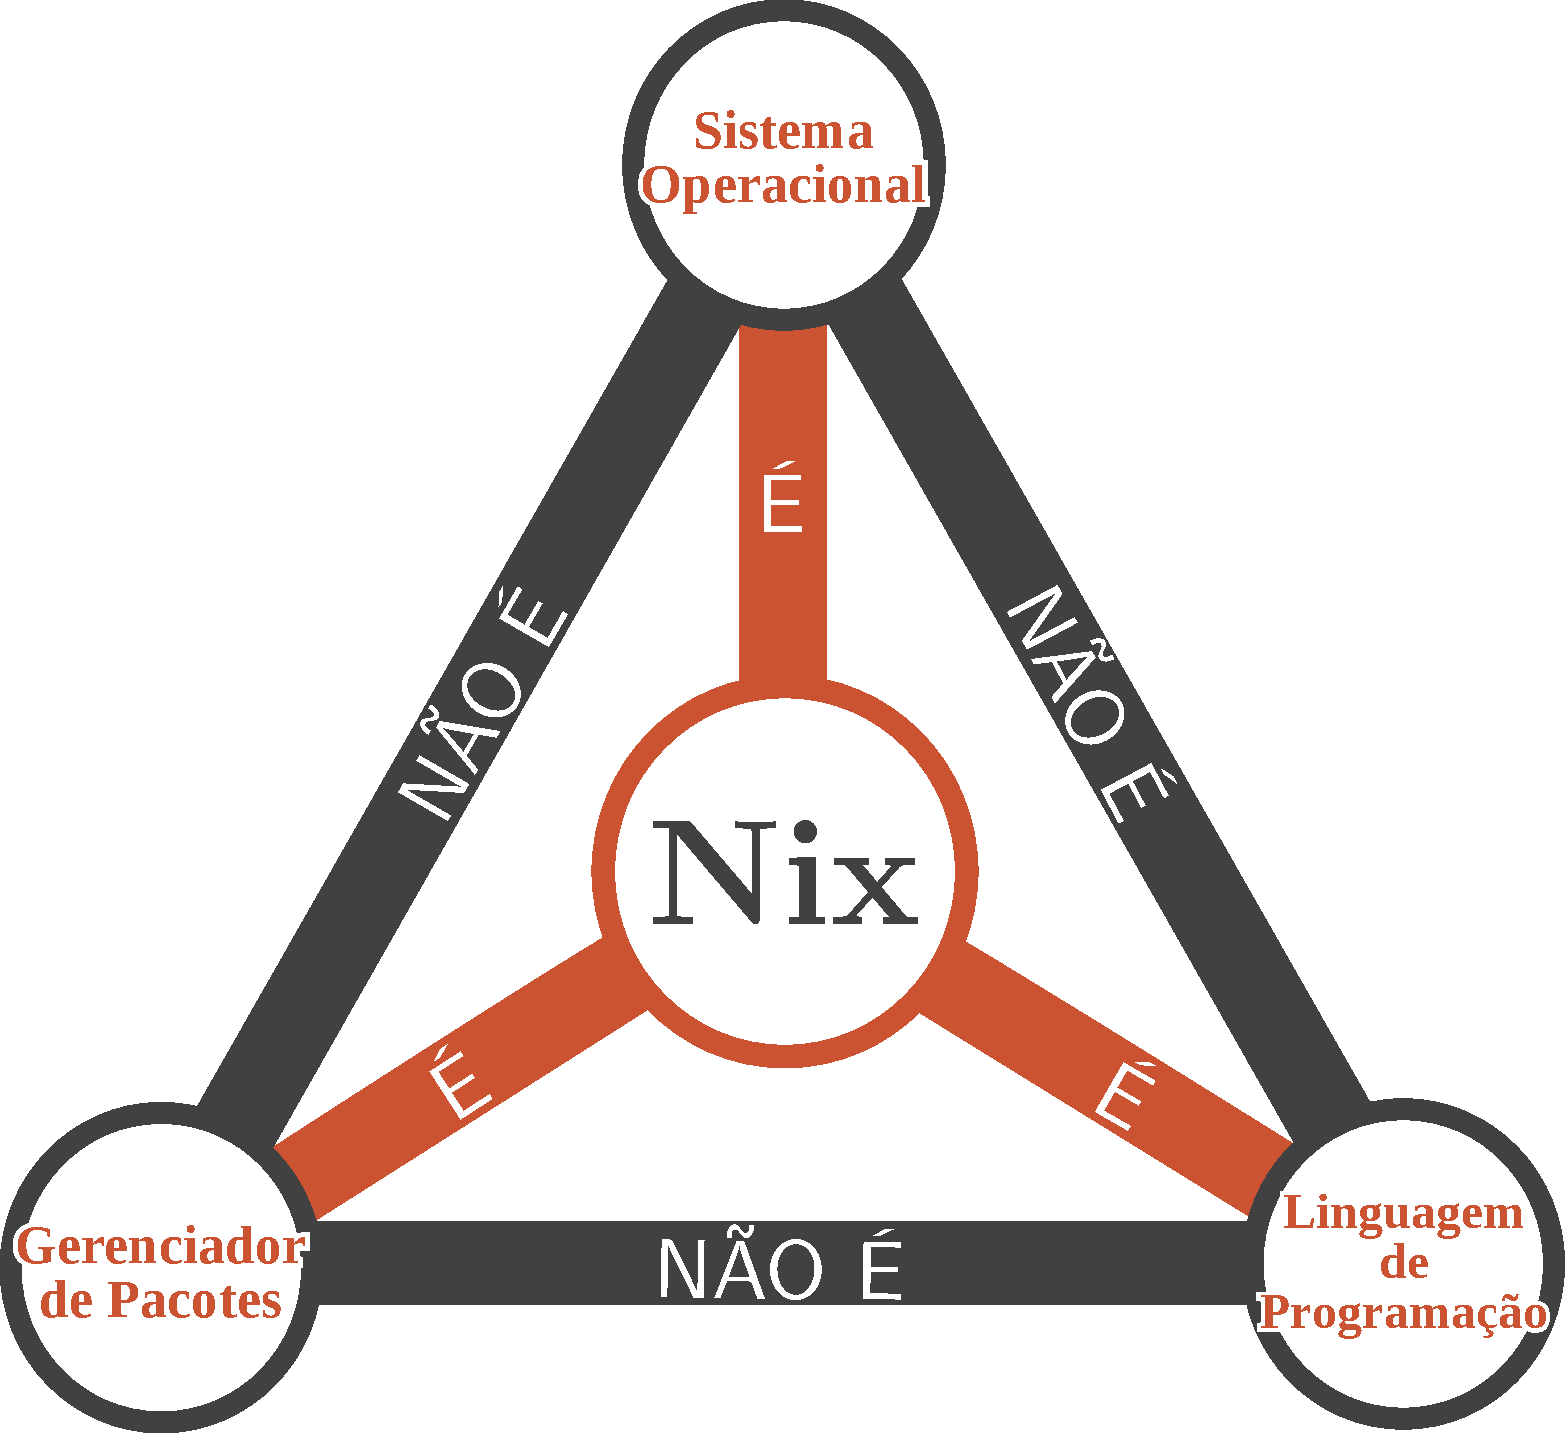
\includegraphics[width=\linewidth]{trinity}
				\par\vspace{-6pt}
				{\scriptsize Fonte: elaborado pelo autor.}
			\end{figure}
		\end{column}

	\end{columns}
\end{frame}

\begin{frame}{A linguagem}
	\small
	Nix é uma linguagem de domínio específico, puramente funcional, de avaliação preguiçosa e tipagem dinâmica \cite{nixdev-language}.

	\begin{description}
		\item[Puramente funcional] um paradigma de programação que trata toda a computação como a avaliação de funções matemáticas, ou seja, funções dependem apenas dos seus argumentos independente de um estado global ou local \cite{wikipedia-functional}. Desta forma, passar uma mesma entrada sempre resulta na mesma saída o que garante determinismo e permite que as derivações sejam hasheadas.
		\item[Avaliação preguiçosa] uma estratégia que adia a avaliação de uma expressão até o seu valor ser necessário e evita repetições por meio de recursos compartilhados \cite{wikipedia-lazy}. Assim, mesmo com um número gigantesco de derivações, o processo de realização de um pacote Nix avalia apenas aquelas que são realmente necessárias.
		\item[Tudo é uma expressão] não há comandos ou instruções: um arquivo \code{.nix} inteiro é avaliado até produzir um único valor.
	\end{description}
\end{frame}

\begin{frame}{Expressões e conjuntos de atributos}
	\begin{columns}[T,onlytextwidth]
		\begin{column}{0.48\textwidth}
			\small\raggedright
			Em Nix, todo arquivo \code{.nix} é uma única expressão e resulta em um único valor. Esse valor costuma ser um \termo{conjunto de atributos} (\en{attribute set}) --- pares de nome e valor acessados por chave --- mas também pode ser um número, uma string, outro tipo primitivo ou uma lista \cite[sec.~Data Types]{nixmanual}.

			\medskip

			Uma \termo{derivação} é simplesmente um conjunto de atributos com uma chave \code{type = "derivation"}.
		\end{column}
		\begin{column}{0.46\textwidth}
			\nixcode{code/attrset}{attrset.nix}
		\end{column}
	\end{columns}
\end{frame}

\begin{frame}{Funções}
	\begin{columns}[T,onlytextwidth]
		\begin{column}{0.44\textwidth}
			\small\raggedright
			O arquivo também pode resultar em uma \termo{função} --- funções são valores como quaisquer outros \cite[sec.~Nix Language]{nixmanual}. Nesse caso, ela recebe um conjunto de atributos como parâmetro para produzir o valor final. Parâmetros podem ter valor padrão (\code{?}).

			\medskip
			O padrão \code{\{ pkgs, versao \}:} não declara dois parâmetros: toda função tem a forma \code{padrão: corpo} e recebe exatamente um argumento --- aqui, um único conjunto de atributos que é desestruturado \cite[sec.~Syntax]{nixmanual}.
		\end{column}
		\begin{column}{0.50\textwidth}
			\nixcode{code/funcao}{funcao.nix}
		\end{column}
	\end{columns}
\end{frame}

\begin{frame}{Aplicação de funções}
	\small
	\begin{columns}[T,onlytextwidth]
		\begin{column}{0.47\textwidth}
			Uma função de \enquote{duas entradas} é, na verdade, uma função que devolve outra função \cite[sec.~Syntax]{nixmanual}.

			\medskip

			\nixcodeinline{code/curry}{curry.nix}
		\end{column}
		\begin{column}{0.47\textwidth}
			Resulta em \code{\{compilador = "gcc-13"; nome = "projeto-raul-2.0"; versao = "2.0"; \}}.
		
			\medskip
		
			\nixcodeinline{code/uso}{uso.nix}
		\end{column}
	\end{columns}
\end{frame}

\begin{frame}{\code{nixpkgs}}
	\begin{columns}[T,onlytextwidth]
		\begin{column}{0.54\textwidth}
			\small\raggedright
			\code{nixpkgs} é o repositório oficial do ecossistema, mantido pela NixOS Foundation junto à comunidade \cite{nixpkgs-manual}.

			\smallskip

			Ele próprio é uma gigantesca expressão Nix: uma função que, ao ser avaliada, devolve um conjunto de atributos com todos os pacotes --- de forma preguiçosa, tal que apenas os pacotes necessários são avaliados.

			\smallskip
			
			Com mais de 100.000 pacotes, é o maior repositório de software do mundo, à frente de AUR, Debian e Homebrew \cite{repology}.

			\smallskip

  			\code{<nixpkgs>} consulta a variável de ambiente \code{NIX\_PATH}, que lista os canais disponíveis na máquina: cópias de repositórios Nix já baixados localmente.
		\end{column}

		\begin{column}{0.44\textwidth}
			\nixcode{code/nixpkgs}{nixpkgs.nix}
	
			\begin{figure}
				\centering
				\begin{tikzpicture}
					\begin{axis}[repobars, symbolic y coords={Homebrew,Fedora,FreeBSD,Debian,AUR,nixpkgs}]
						\addplot[fill=barlo,draw=none] coordinates {(8351,Homebrew) (22482,Fedora) (33440,FreeBSD) (41610,Debian) (95357,AUR)};
						\addplot[fill=barhi,draw=none] coordinates {(119028,nixpkgs)};
					\end{axis}
				\end{tikzpicture}
				\caption{Projetos por repositório em 4 out.\ 2026}
				\label{fig:repos}
				\vspace{-11pt}
				{\scriptsize Fonte: \textcite{repology}.}
			\end{figure}
		\end{column}

	\end{columns}
\end{frame}

\begin{frame}{\code{builtins} e \code{lib}}
	\begin{columns}[T,onlytextwidth]
		\begin{column}{0.42\textwidth}
			\small\raggedright
			\code{builtins} são as funções primitivas embutidas no avaliador, implementadas em C++. A biblioteca padrão de Nix é \code{lib}: um atributo de \code{nixpkgs} escrito inteiramente em Nix, sobre esses \code{builtins} \cite{nixpkgs-manual}.

			\medskip

			\code{lib} cobre listas, conjuntos de atributos, strings, licenças e o sistema de módulos de NixOS.
		\end{column}
		\begin{column}{0.54\textwidth}
			\nixcode{code/lib}{lib.nix}
		\end{column}
	\end{columns}
\end{frame}

\begin{frame}{Funções de alto nível}
	\begin{columns}[T,onlytextwidth]
		\begin{column}{0.42\textwidth}
			\small\raggedright
			Sobre essas primitivas, \code{nixpkgs} constrói funções que encapsulam tarefas inteiras. Elas residem em \code{pkgs}, não em \code{lib}.

			\smallskip

			Os \termo{fetchers} baixam uma fonte e a verificam por hash para segurança e reproducibilidade; os \termo{builders} por linguagem resumem toda a cadeia de compilação em uma única chamada.

			\smallskip

			\code{pacote.nix} não importa nenhuma delas: apenas declara o que precisa como parâmetros. É \code{callPackage} que lê esses nomes e injeta os atributos de mesmo nome vindos de \code{pkgs}.
		\end{column}
		\begin{column}{0.54\textwidth}
			\nixcode{code/pacote}{pacote.nix}
		\end{column}
	\end{columns}
\end{frame}

\begin{frame}[allowframebreaks,t]{Referências}
	\printbibliography[heading=none]
\end{frame}

\end{document}
